%%
%% Larson Hogstrom 
%% MIT 18.335
%% Final Project
%% 5/12/2015

\documentclass[final,leqno,onefignum,onetabnum]{siamltex1213}

\usepackage{algorithm2e}
\usepackage{amsmath}
\usepackage{cite}

\usepackage{graphicx}
%% \graphicspath{ {"/Users/hogstrom/Dropbox (Personal)/cources_spring_2015_MIT/18_335_Numeric_Methods/NMF/figures/"} }
\graphicspath{ {/Users/hogstrom/Documents/code/ThornsInRoses/18_335} }
\DeclareGraphicsExtensions{.pdf,.png,.jpg}

\title{Numeric methods for Nonnegative matrix factorization \thanks{A final project for 18.335, Spring 2015}} 

\author{Larson Hogstrom\thanks{
(\email{hogstrom@mit.edu}). }}


\begin{document}

\maketitle
\slugger{mms}{xxxx}{xx}{x}{x--x}%slugger should be set to mms, siap, sicomp, sicon, sidma, sima, simax, sinum, siopt, sisc, or sirev

\begin{abstract}
C This report presents a framework and analysis to compare three common methods for computing nonnegative matrix factorization (NMF). The parts-based representation obtained through NMF has become a popular approach for dimensionality reduction in a variety of scientific and technical domain. This study focuses on the algorithms and numerical aspects of NMF computation. We review the derivation and continual descent properties of the multiplicative update rules which helped to first popularized the NMF approach. Alternating least squares and projection gradient methods are also presented as faster, more recent approaches. The accuracy and convergence of these algorithms is compared using simulated data and two of the methods were applied to a database of gene expression profiles measuring drug responses in the MCF7 cancer cell line. Lastly, the objective function of alternating least squares was directly modified to impose sparsity during matrix factorization. The fraction of near-zero entries was compared before and after ALS modification as sparsity results are of known interest to many researchers using NMF. 
\end{abstract}

\begin{keywords} dimensionality reduction, matrix factorization, least squares, nonnegativity, data representation \end{keywords}



\pagestyle{myheadings}
\thispagestyle{plain}
\markboth{18.335 FINAL REPORT}{Numeric methods for nonnegative matrix factorization}

\section{Introduction}

Non-negative data is pervasive in many domains. Chemical concentrations, word counts from written text, and pixels in digital images all take strictly non-negative values. Researchers working with these and related datatypes often seek to manipulate and interpret large matrices of input data. Low-rank approximations can aid in identifying the most important components of such data by ignoring nonessential components related to noise or known artifacts. Common goals in performing such low-rank approximations include clustering similar items into groups, retrieving related samples based on an user's input query, or isolating representative components of the data that can be directly interpreted \cite{Lan}.  

Nonnegative matrix factorization (NMF) is a dimensionality reduction technique that  has been employed to address a variety of scientific and engineering challenges including text data mining \cite{Pau,Lan,LeSe1} chemometrics \cite{Paa1,Paa2}, and microarray analysis \cite{Bur}. Like principal component analysis (PCA), NMF seeks to describe a large matrix of data using a small set of information dense components. Unlike PCA, which imposes orthogonality constraints on components, NMF requires nonnegativity after factorization. This procedure allows for only additive combinations of positive components to estimate the input matrix. The endpoint is a parts-based representation of the starting data where each component is more easily interpreted than PCA. 

A number of algorithms have been proposed in order to construct NMF factorization with non-negative constraints. This approach was largely popularized by a 1999 article by Lee and Seung \cite{LeSe1}. Their study, written for a general audience, examined the benefits of parts-based representations and presented applications of NMF to domains including text analysis and the decomposition of facial images. The report was followed by an additional study outlining more mathematical details of NMF as well as a simple multiplicative update algorithm \cite{LeSe2}. The publications of Lee and Seung, however, were predated by lesser known work by Pentti Paatero. The method he developed and named 'positive matrix factorization' was based on a constrained alternating least squares algorithm and represents the first presentation of what is today known as NMF \cite{Paa1,Paa2}. 



To date, 
Iterative algorithms, for example, build factorized components while converging on a local minimum of a specified object function. 

-problem with NMF - no unique solution 
In NMF, a low ran approximation of an input data matrix A is created with smaller, non-negative factors called W and H. 
In the case of gene expression and other biological phenomena 

This project compares multiple algorithms for computing NMF factorization including gradient and non gradient methods. The motivation 
fixed-point type methods 
minimization problem with bounded constraints 

For the purposes of this study, algorithms are implemented and evaluated in the python language using the 'numpy' and 'scipy' packages for scientific computation. In simulations, the algorithms are compared by their accuracy after a fixed number of iterations. To illustrate a real-world applications of NMF, non-negative, low-rank approximations were used to describe gene expression profiles of known pharmacological groups. This proceeding report is organized in the following structure. Section 2 defines the NMF approach and reviews commonly used objective functions. Section 3 outlines the multiplicative update rule which is one of the oldest and most widely used procedures to perform matrix decomposition with NMF. Section 4 covers the alternating least squares approach which variations with better characterized convergence properties. This is followed by a discussion of sparsity and initialization conditions. 

\section{Problem Definition and Objective Functions}

\begin{definition} For a nonnegative matrix $\textbf{A} \in \Re^{m x n} $, select a low-rank approximation of size k such that there are two nonnegative matrices \textbf{W} $ \in \Re^{m x k}$ and \textbf{H} $ \in \Re^{k x n}$ which minimizes a function such as 
\begin{equation}\label{ObjEuc}
 f( \textbf{W,H}) = \frac{1}{2} || \textbf{A - WH} || ^{2}_{F}
\end{equation}

\end{definition}

KKT optimality conditions a stationary point for 




Other commonly used objective functions include Euclidian distance and Kullback-Leibler (KL) divergence. KL can be extended to a more general information-based framework using Renyi's divergence \cite{Dev1}. Here, a single parameter $\alpha$ is used to represent a continuum of distance measures and KL airises as a special case as $\alpha \to 1$. 
\begin{equation}\label{ObjKL}
 KL(A || WH) = \sum_{ij}{[A_{ij} \log{ \frac{A_{ij}}{(WH)_{ij}} - A_{ij} + (WH)_{ij}} ]}
\end{equation}
For its simplicity and widespread use, this report will focus on objective function defined in (2.1). 

Regardless of the objective used to obtain them, the resulting W and H matrices are often interpreted directly. The matrix \textbf{W} $ \in \Re^{m x k}$ typically represents the k different components of signal in the original matrix. The \textbf{H} $ \in \Re^{k x n}$ matrix can be interpreted as weighting factors defining the linear combination of k components used to reconstruct a sample in the original data matrix. In the application of NMF to gene expression data for example, each of the k columns of W represent a 'metagene' response. A small number of these metagene columns can be combined to estimate an original experimental column found in the original data matrix. The H matrix defines the weighting of each metagene. 


\section{Multiplicative Update Rule} In their seminal paper, Lee and Seung began their analysis with a simple additive update rule for H that reduces the squared distance: 
\begin{equation}\label{au1}
 H_{aj} \leftarrow  H_{aj} + \eta_{aj} [ (W^T A)_{aj} - (W^T WH)_{aj}]
\end{equation}

The authors noted that this update represents a typical gradient descent rule if each of the $\eta_{au} $ terms are all equally set to a small positive number. Alternatively, the variables can be diagonally rescaled by setting
\begin{equation}\label{et1}
 \eta_{aj} = \frac{ H_{aj} }{(W^T WH)_{aj}}
\end{equation}
and when placed into equation (3.1), this motivates the multiplicative update rules that seek to minimize the euclidian distance $||A - WH ||$:
\begin{equation}\label{au1}
 H_{aj} \leftarrow  H_{aj} \frac{(W^T A)_{aj} }{ (W^T WH)_{aj} } \; \; \; \; \; W_{ia} \leftarrow  W_{ia} \frac{(W^T A)_{ia} }{ (W^T WH)_{ia} }
\end{equation}
Where the same logic for H is also applied to the update of W. Making use of auxiliary functions, Lee and Seung went on to demonstrate the non-increasing properties of NMF under the multiplicative update rules. It has been noted that they incorrectly claimed that algorithm converges to a local minimum \cite{Chu, Gon, Lin}. It is certainly possible that continual descent property of multiplicative updates could descend to a saddle point \cite{Ber}. Furthermore, if $W_{ia} = 0$ after the $k$th iteration, then this entry remains $W_{ia} = 0$ for all subsequent iterations. This property is undesirable because the algorithm could theoretically remain fixed in a non-optimal descent path. \\

\begin{algorithm}[H]
 \KwData{Input data matrix:  $\bf{A} \in \Re^{m x n}$}
 \KwResult{nonnegative factorization of \textbf{A} using k components, creating matrices \textbf{W} $ \in \Re^{m x k}$ and \textbf{H} $ \in \Re^{k x n}$ }

 initialization\;
$\bf{W} \gets $ random dense (m x k) matrix\\
$\bf{H} \gets $ random dense (k x n) matrix\\
 \For{i = 1 to \text{maxiter} }{
 	$\bf{H = H .* (W^T A) ./ (W^T WH)} $
	
 	$\bf{W = W .* (A H^T) ./ (WHH^T)} $	}
 \caption{Multiplicative update}
\end{algorithm} 

It is important to note that this approach will breakdown if a zero appears in the denominator. In practice, it is common to add a very small floating point value to the denominator during each iteration. The required work of O(mnk) per iteration is quite high compared to other exiting algorithms and multiplicative update tends to converge slowly for real world problems. Nevertheless, with its early establishment and its straightforward implementation this algorithm has maintained popularity for NMF computation. 

\section{Alternating Least Squares} The alternating least squares can be viewed as a special case of block coordinate descent method. For this class of algorithms, the objective function is minimized with respect to coordinate vectors $x^{k}_{i}$. Multidimensional vectors are minimized in cyclical order, with one block coordinate vector minimized during each iteration (Berstekas, 1999). A single iteration takes the form:
\begin{equation}\label{bcv1}
 x^{k+1}_{i} \in {\mathrm{argmin}_{\varepsilon \in X_i}} = f( x^{k+1}_{1}, ..., x^{k+1}_{i-1}, \varepsilon, x^{k}_{i+1}, ..., x^{k}_{n})
\end{equation}
For the case of NMF, this scenario is especially simple as there are only two block variables, W and H. Sequentially one matrix is fixed and the other is improved. 

\begin{equation}\label{bcv2}
W^{k+1} = {\mathrm{argmin}_{W \ge 0} f(W,H^k}) \\
H^{k+1} = {\mathrm{argmin}_{H \ge 0} f(W^{k+1},H})
\end{equation}




This takes advantage of the fact that while objective (2.1) is not convex in both W and H, it is convex in either W or H individually. One basic least ALS algorithm to accomplish this outlined by Berry et al \cite{Ber}. This strategy imposes nonnegativity by setting all nonzero entries of W and H to zero during each iteration. Unlike multiplicative update rules, however these zero entries are not forced to remain at 0 for all proceeding iterations. \\

\begin{algorithm}[H]	
 \KwData{Input data matrix:  $\bf{A} \in \Re^{m x n}$}
 \KwResult{nonnegative factorization of \textbf{A} using k components, creating matrices \textbf{W} $ \in \Re^{m x k}$ and \textbf{H} $ \in \Re^{k x n}$ }

 initialization\;
$\bf{W} \gets $ random dense (m x k) matrix\\
$\bf{H} \gets $ random dense (k x n) matrix\\
 \For{i = 1 to \text{maxiter} }{
 	Solve for $\bf{H}$ in $\bf{W^T WH = W^T A} $
	
	set negative elements in $\bf{H}$ to 0
	
 	Solve for $\bf{W}$ in $\bf{HH^T W^T = HA^T}$
	
	set negative elements in $\bf{W}$ to 0	}
 \caption{Alternating least squares}
\end{algorithm} 

Each subproblem from in this algorithm is solved in an unconstrained manner and the resulting W and H solutions are modified during each iteration to satisfy the desired non-negativty constraints. The simplicity of setting negative values in W and H to zero provides for an especially fast approach as demonstrated in the comparisons of this study. Theoretical evaluation of this algorithm's convergence properties, however, are difficult because each subproblem is formulated as an unconstrained least squares problem, but the solutions are directly modified and therefore do not map onto the original formulations. Other problem definitions allow for a framework to better understand the convergence properties of the two block coordinate descent method. Alternating non-negativity constrained least squares (ANLS) for instance provides a formulation that directly incorporates non-negative constraints in each block coordinate subproblem \cit{Kim1}. Adding the $W \ge 0$ and  $ H \ge 0 $ constraints onto equations () and () respectively, the Karush-Kuh-Tucker (KK) optimality conditions can be used to define stationary points of the objective function (2.1) iif
\begin{equation}\label{EKx}
 \begin{align}
  W \ge 0,\\
  \bigtriangledown_W f(W,H)  = WHH^T - AH^T \ge 0,\\
  W.* \bigtriangledown_Wf(W,H) = 0\\ \\
    H \ge 0,\\ 
  \bigtriangledown_H f(W,H)  = W^T WH - W^T A \ge 0,\\
  H.* \bigtriangledown_Hf(W,H) = 0  
  \end{align}
\end{equation}

For the block coordinate descent algorithms, it has been shown that the limit point of a sequence of sub-blocks is a stationary point if each subproblem has a unique solution \cite{Ber2}. Unfortunately, ANLS subproblems are not unique as there exists matrices in the form $ \textbf{X} \in \Re^{kxk} $ which represent scaling and permutation that satisfy $ || \textbf{A - WH} ||_{F} = || \textbf{A - WXX}^{-1} \textbf{H} ||_{F} $ \cite{Kim1}.  In the case of two bock problems, however, stationary points can be found as the limit point of the sequence of two sub-block solutions \cite{Gri}. One classical approach to solving the two block subploblems is by way of an $\textit{active set algorithm}$ (Lawson, 1974). Here, the difference between a input matrix $ Y \in \Re^{lxp}$  and its resultant factorization cab be split into vectors:

\begin{equation}
    \min_{G \ge 0} || BG-Y ||^{2}_{F} \to  \min_{G \ge 0} || B\textbf{g}_1-\textbf{y}_1 ||^{2}_{2}, ...,   \min_{G \ge 0} || B\textbf{g}_l-\textbf{y}_m ||^{2}_{2}
\end{equation}

where $ B \in \Re^{lxm}$ and $y_i \in \Re^{lx1}$. Since there are m inequity constraints after the split, the ith constraint will be active if the ith regression coefficient is set to zero. Thus if the active set is known, active constraints can be treated as equality constraints instead of inequality constraints. The overall least square problem can be solved by examining only the variables in the passive set and calculating their unconstrained least squares solution (Bro, 1997). The ANLS algorithm begins with an initial feasible set of regression coefficients. The zero vector of coefficients is often used as an initial feasible set as no constraints are violated. ANLS proceeds by iteratively removing variables from the active set until the true active set is found. The variables removed from the active set are used in an unconstrained linear regression to calculate the block coordinate descent solution. While the convergence properties of ANLS are better understood, this report omits this strategy in comparative analysis due to the complexity of the algorithm and its slow computation. Recent work has succeeded in improving ANLS speed by precomputing cross-product terms during the unconstrained linear regression calculations (Bro, 1997). 

\section{Sparsity in Alternating Least Squares} The sparsity of 

The two potential benefits of increasing sparsity in NMF representations. First, there is potential for saving storage and future computation relative to dense representations that occur with dense factorization methods such as SVD. Second and more importantly, sparsity may aid in interpreting the NMF results. 

To better control the fraction of zero or near zero entries, Kim and Park propose directly modifying The objective function of the ALS method. 
\begin{equation}\label{ObjSpar}
 f( \W,H) = \frac{1}{2} [|| A - WH ||^{2}_{F} + \lambda_W || W ||^{2}_{F} + \lambda_H || H ||^{2}_{F} ]
\end{equation}
Here additional terms are used to 
Added penalties to objective function to encourage sparse solutions. Xxx

This can be easily incorporated into the two block coordinate framework 
\begin{equation}
    \min_{W \ge 0} || \left( \begin{array}{c} H^T   \\  \sqrt{\alpha_W}I_k \\ \end{array} \right) W^T- \left( \begin{array}{c} A^T   \\  0_{kxm} \\ \end{array} \right) ||^{2}_{F} 
\end{equation}
where $I_k$ is the $k\text{ x }k$ identity matrix and  $0_k$ is a zero matrix with the size $k\text{ x }m$
\begin{equation}
    \min_{H \ge 0} || \left( \begin{array}{c} W   \\  \sqrt{\alpha_H}I_k \\ \end{array} \right) H- \left( \begin{array}{c} A   \\  0_{kxm} \\ \end{array} \right) ||^{2}_{F} 
\end{equation}

\begin{figure}[h!]
  \centering
    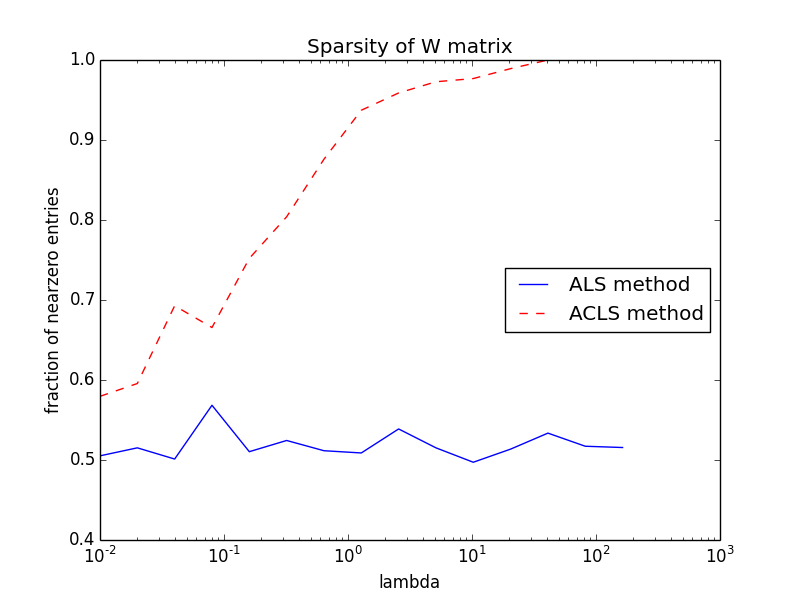
\includegraphics[width=.5\linewidth]{ALS_vs_ACLS_sparsity}
  \caption{NMF sparsity manipulation using the ACLS method. Increasing the value of $\lambda$ allows users to increase the fraction of near-zero entries in W and H.}
\end{figure}


\section{Projection gradient method} 


\section{Applications to gene expression}
A classical example of NMF is the factorization of a large database of human face images. Factorization using PCA will yield a series of ?eigenfaces? which can be added or subtracted, but individual components are not easy to interpret on their own. The NMF "parts-based" representation however, yields components like noses, eyes, ears, and mouths which can be added linearly to construct a face. Parts-based representations have been helpful in identifying and interpreting patterns in a number of biological contexts. 

NMF has shown to be less sensitive to \textit{a priori} gene selection or initial conditions when identifying context-dependent patterns of gene expression (Brunet, 2004). 

The same properties have been found to be helpful in a number of biological contexts. 

The similar results found with ALS and gradient projection, point to the importance of other factors. The effects of sparsity were not examined with this particular dataset, but could have a significantly influence on the interpretation of the NMF results. Other factors, including smoothness, ____ and ___ could also impact the 

\section{Initialization conditions}

\section{Additional computational issues}
-Sparsity 

\section{Conclusion} Despite the simplicity of defining nonnegative matrix factorization, the landscape of numeric methods used to address the problem remains complex. Recent efforts have sought to create new NMF algorithms with well defined convergence properties. Methods such as alternating non-negativity constrained least squares (ANLS) have succeeded in improving our analytical understanding of NMF convergence, but remain slow and cumbersome when compared to simpler methods that appear to converge in most real-world scenarios. When evaluating NMF tools, researchers should be guided by the parameters of their data and the research question of interest. For especially large datasets the speed and simplicity ALS might serve as a reasonable starting point for NMF calculation. Researchers with modest datasets, might prefer ___ . The results presented in this report also show that researchers can manipulate the sparsity of factorization by adopting specialized objective functions. 

\begin{thebibliography}{1}

\bibitem{Lan} {\sc A. Langville, C. Meyer, R. Albright},
{\em Initializations for the nonnegative matrix factorization}, Preprint (2006) 

\bibitem{Pau} {\sc V Pauca et al},
{\em Text mining using non-negative matrix factorizations}, Proceedings SIAM International Conference on Data Mining (2004) SDM'04. 

\bibitem{Paa1} {\sc P. Paatero},
{\em Positive matrix factorization; a non-negative factor model with optimal utilization of error estimates of data values}, Environmetrics (1994) 5, 111-126.

\bibitem{Paa2} {\sc P. Paatero},
{\em Least squares formulation of robust non-negative factor analysis}, Chemometrics and Intell. Laboratory Syst. (1997) 37, 23-35.

\bibitem{Paa3} {\sc P. Paatero},
{\em The multilinear engine - a table-driven least squares program for solving multilinear problems, including the n-way parallel factor analysis model}, J. Comput. Graphical Statist. (1999) 8, 1-35.

\bibitem{LeSe1} {\sc D. Lee, H. Seung},
{\em Learning the parts of objects by non-negative matrix factorization}, Nature (1999) 401, 788-791.

\bibitem{LeSe2} {\sc D. Lee, H. Seung},
{\em Algorithms for Nonnegative Matrix Factorization}, Advances in Neural Information Processing Systems (2001) 13, 556-562.

\bibitem{Bur} {\sc J. Brunet et al. },
{\em Metagenes and molecular pattern discovery using matrix factorization}, Proceedings of the Nat. Acad. Sci (2004) 101, 4164-4169. 

\bibitem{Dev1} {\sc K. Devarajan, K. Ebrahimi },
{\em Molecular pattern discovery using non-negative matrix factorization based on Renyi's information measure}, Preprint (2005)

\bibitem{Chu} {\sc M. Chu, D. Plemmons, S. Ragni},
{\em Optimality, computation, and interpretation of nonnegative matrix factorizations},  SIAM Journal on Matrix Analysis (2004)

\bibitem{Gon} {\sc E. Gonzalez, Y. Zhang},
{\em Accelerating the lee-swung algorithm for nonnegative matrix factorization}, Technical Report TR-05-02, Rice University (2005)

\bibitem{Lin} {\sc C. Lin},
{\em Projected gradient methods for non-negative matrix factorization}, Information and Support Services Technical Report (2005)

\bibitem{Ber} {\sc M. Berry, M. Browne, A. Langville, P. Pauca, R. Plemenos},
{\em Algorithms and applications for approximate nonnegative matrix factorization}, Computational Statistics and Data Analysis 52 (2007) pp. 155 - 173.

\bibitem{Ber2} {\sc D. Bertsekas},
{\em Nonlinear Programing}, Athena Scientific, Belmont, MA (1999)

\bibitem{Gri} {\sc L. Grippo et al.},
{\em On the convergence of the block nonlinear Gauss-Seidel method under convex constraints}, Oper. Res. Lett (2000) 26(3), p. 127-136.

\bibitem{Law} {\sc C. Lawson, R. Hanson},
{\em Solving Least Squares Problems}, SIAM, Philadelphia, PA (1995)

\bibitem{Bro} {\sc R. Bro, S. Jong},
{\em A fast non-negativity constrained linear least squares algorithm}, J. Chemometrics (1997) 11), p. 393-401.

\bibitem{Cic} {\sc A. Cichocki, R. Zdunek, A. Huy Phan, S. Amari}, {\em Nonnegative Matrix and Tensor Factorizations}, Wiley, Natick, MA, 2009.

\bibitem{Kim1} {\sc H. Kim, H. Park}, {\em Nonnegative matrix factorization based on alternating nonnegativity constrained least squares and active set method}, SIAM Journal on Matrix Analysis and Applications (2008) 30(2), 713?730.

\bibitem{Kim2} {\sc H. Kim, H. Park}, {\em Sparse non-negative matrix factorizations via alternating non-negativity-constrained least squares for microarray data analysis}, Bioinformatics (2007) 23, 1495-1502. 

\bibitem{Alb} {\sc R. Albright, J. Cox, et al.},
{\em Algorithms, initializations, and convergence for the nonnegative matrix factorization}, Preprint (2014)

\bibitem{Lin} {\sc C. Lin},
{\em Projected Gradient Methods for Nonnegative Matrix Factorization}, Neural Computation (2007) 19, 2757-2779. 

\end{thebibliography}


\end{document}
%% end of file `docultex.tex'
